\chapter{Design}
coming from previous chapter: Code Restructuring; Data Restructuring; Forward Engineering
    
    
explain the internal design of the new application.
internal design of the application. this should be the fun part.

\section{Technology}
angularJS (teach the browser new syntax), javascript, html5, Qt, QtBrowser and its limitations (JS engine vs chrome v8 or firefox's). tdd+jasmine

The project of this thesis, Flango Content Manager, is designed to work client side in a web browser.
The natural technology in this environment is JavaScript, HTML and CSS.
It interoperates with other systems that feature a different technology. FIXME CROSS REF PHYISICAL DESIGN or CONTEXT



\subsection{JavaScript}
some hints. functional. scopes.
language, jquery, qr, swf

Object Literal Notation, constructors, closures, var scope, concept of classes
notes:

First thing you need to know is that JavaScript uses prototype-based inheritance. This means there is no distinction between classes and instances as in other OO languages (like Java). There are just objects. One implication of that is that differentiating between class and object diagrams does not make sense.

Keep in mind that UML includes many types of diagrams, specifically a branch of behavior diagrams, including sequence and use case diagrams. Such diagrams specifically address your concern of modeling javascript as a behavior driven language.

It is quite possible that a javascript system is not using object-oriented design. In such a case, class diagrams would probably not be appropriate, as you pointed out. However, since javascript does support object-oriented design, it is possible for class diagrams to effectively depict a system using javascript. It really depends on how the javascript is being used.

JavaScript is an
object-based
language. Just as in C\#, you can create objects, call their
methods, pass them as parameters, and so on. You could see this clearly when working
with the DOM, where you manipulated the HTML document through the methods
and properties of the implicit
document
object. However, JavaScript isn't generally
considered a fully object-oriented language because it lacks support for some features
that you'd
fi
nd in "real" OOP languages, or simply implements them differently.

 What does "object-oriented programming" mean anyway? Basically, as the name
suggests, OOP puts objects at the centre of the programming model. The
object
is
probably the most important concept in the world of OOP—a self-contained entity
that has
state
and
behavior
, just like a real-world object. Each object is an instance of a
class
(also called
type
), which de
fi
nes the behavior that is shared by all its objects


******
description of the language and big uses
objects
functions
prototypal inheritance (vs classical model, new, etc)


\subsection{AngularJS}
about the framework. directives, services, 
The framework enforces a very strict separation of responsibilities: \ac{DOM} updates are abstracted away from model updates. 
Directives act as the layer that keeps these two aspects loosely coupled.
One one hand, directives translate data into user interfaces and, on the other hand, directives translate user interactions back into \$scope behaviors. FIXME Reword this

\paragraph{Overview} AngularJS is a framework for dynamic web applications.
\ac{HTML} was created to declare static documents and needs libraries and frameworks to enable application development.
Angular lets developers use \ac{HTML} in the templates and extend the language syntax to express reusable components.
It \textit{teaches the browser new syntax} through a construct called Directive.
Features:
\begin{itemize}
    \item Tools to build \ac{CRUD} Applications: data-binding, basic templating directives, form validation, routing, deep-linking, reusable components, dependency injection.
    \item Tools to test: unit-testing, end-to-end testing, mocks.
\end{itemize}

Flango Content Manager reads \ac{XML} and renders it as \ac{HTML}.
There are two possible approaches: parsing the \ac{DOM} tree in the browser or teaching the browser new syntax.
This project uses the second (FIXME language: the latter?): instead of developing an algorithm to traverse the tree and render elements, it defines reusable components (AngularJS Directives) and includes the \ac{XML} files in the appropriate place in the \ac{DOM}. 
The browser already traverses the tree to render the page and there is no need to do it manually.
Normally a browser ignores an element that doesn't belong to the \ac{HTML} specification (e.g. \lstinline$<fl:ui fl:type="base-button"></ui>$)
With AngularJS, the browser runs the behaviour defined in the reusable component.

\paragraph{Building Blocks} There are several key components in AngularJS to build the application.

\begin{itemize}
    \item Controller: a function that binds the view with the model. It typically assigns objects to the \$scope variable to expose them to the template.
    \item Directive: a construct to extend HTML with custom attributes and elements. It defines the template of the reusable component, the behaviour, the attributes, etc. For instance, the directive $flBaseButton$ states that the node $<fl:ui fl:type="base-button">$ in the \ac{DOM} tree should be transformed into a simple $button$ using the theme template $baseButton.xml$. 
    \item Service: Singleton that encapsulates reusable business logic independent of views. For instance, a service to handle the configuration of the application. They can be injected in controllers, directives or other services.
    \item Filter: a function that formats the value of an expression for display to the user. For instance, a filter to display a Number with currency format.
    \item Module: These building blocks are grouped in Modules. They can have dependencies between them.
\end{itemize}

The framework provides all the necessary tools to use unit and end-to-end testing from the very beginning of the project.
Considering testing as equal in importance to application writing makes the code to be more robust, lowers the cost of maintenance and helps to have a better internal design.
\begin{itemize}
    \item Jasmine is a behavior-driven development framework for testing JavaScript code. It does not depend on any other framework and does not require a \ac{DOM}. It provides a simple, self-descriptive (FIXME language!) syntax to write test suites.
    \item Angular Mocks: there are stub objects ready to load in tests (e.g. \$httpBackend mocks \ac{HTTP} calls)
    \item Karma is a test runner to automate the execution of the test suites. 
\end{itemize}
    
\paragraph{Compile-Link} To make directives possible Angular has a compiler.
In this context, compiling means attaching event listeners to the \ac{HTML} to make it interactive.
The compiler traverses the \ac{DOM} tree in two phases:
Firstly it looks for tags that have directives associated (e.g. $<fl:ui fl:type="base-button">$ or even native \ac{HTML} elements $<a>$).
Secondly it binds the model to the view.
The compiler allows developers to attach behaviour to any \ac{HTML} element or attribute and even create new HTML elements or attributes with custom behaviour. Angular calls these behaviour extensions directives.

\paragraph{Directive} At a high level, directives are markers on a \ac{DOM} element (such as an attribute, element name, \ac{CSS} class or a comment) that tell Angular's \ac{HTML} compiler to attach a specified behaviour to it or even replace it with another element.
The \ac{HTML} compiler finds elements that match directives. 
For example, for $<div ng-controller="myCtrl">$, the element $div$ matches the directive $ngController$.
An example in Flango Content Manager: when the browser finds $<fl:width>150</fl:width>$ in the \ac{DOM}, the element $width$ matches the directive $flWidth$.
The $flWidth$ directive is restricted to elements (it matches $<fl:width>150</fl:width>$ but not $<div fl:width>150</div>$ because it is an attribute), and it has a custom $link$ function that performs some computation.

    
\subsection{HTML5}
maybe not useful. maybe just html

\subsection{SASS}
Writing plain \ac{CSS} can be tedious and error-prone.
SASS stands for Syntactically Awesome CSS and is a pre-processor with syntax advancements that add features to \ac{CSS}.
Sass is an extension of \ac{CSS}3, adding nested rules, variables, mixins, selector inheritance, and more.
It is then translated into well-formated, standard \ac{CSS} using the command line tool.
This makes reusing and extending \ac{CSS} easier.
SASS has two syntaxes. This project uses the newest one, known as \ac{SCSS} (Sassy CSS).

A key feature in this project is the "$@extend$" directive: it tells SASS that one selector should inherit styles of another selector.
Example: the style $base-button$ has a grey background. The style $button$ sets the size of the element to $100 x 50 px$.
Because all $base-button$s are $button$s, a $base-button$ should inherit the style from $button$ instead of replicating it, like one would do with \ac{OOD} in a programming language.
With \ac{HTML} this would be written $<div class="base-button button" />$.
With SASS one can write $.base-button { @extend .button }$ and keep \ac{HTML} cleaner: $<div class="base-button" />$

SASS variables and mixins make it easier to scaffold (FIXME LANGUAGE!) themes for Flango Content Manager and have consistency in the visual design (e.g. all themes can have palettes of the same size).

\subsection{Robot Web Tools}
Robot Web Tools is a collection of open-source modules and tools for building web-based robot applications.
It provides 3 core libraries to communicate with \ac{ROS} on the robot over rosbridge's WebSocket server: roslibjs, ros2js, and ros3djs.
This project uses roslibjs to subscribe and publish to Topics.

\section{Architecture}
context: comm with rob behaviour and rostopics (SOA).
MVC. client-side. JSON to talk to an API. xml files as angularjs partials, hacks to make it work (routes defined manually, one controller for all of them, dirty entities). scopes and their specific use here (compare to regular use). what about MVVM?

common patterns:
dependency injection and angularJS (and literature: fowler)

\subsection{Context}
Flango Content Manager is a piece in the robot.
\ac{ROS} is a framework for robot software development that provides operating system-like functionality on a heterogeneous computer cluster. 
It was originally developed in 2007 as part of the Stanford AI Robot (STAIR) project with the goal of providing an architectural framework supporting modular, tool-based development for robotic software.
It has a loosely coupled architecture with nodes, messages, topics and services, similar to \ac{SOA}.

DIAGRAM HERE: rosmaster (service registry), services, topics

Nodes are processes that perform computation, a "software module". 
Nodes communicate with Messages, strictly typed data structures . There are some available by default, like $std_msgs/String$ and other primitive types.
Nodes subscribe and publish to topics, identified by a name (string).
Services are pairs of request/response messages offered in a node designed for simple synchronous transactions.
FIXME add ActionServers???


http://www.willowgarage.com/sites/default/files/icraoss09-ROS.pdf

The robot has two parts: robotBehaviour and Stacks.
Part of the code of the robot (robotBehaviour) does not follow the \ac{ROS} workflow but still uses Topics to communicate with the Stacks, the part of the project that does use \ac{ROS}.
In Stacks there are Servers and ActionServers that provide Services.
Flango is a component in this system that communicates with robotBehaviour using \ac{ROS} Topics and two types of messages.
It is not designed strictly as a service to handle synchronous requests but it is able to use Topics to have asynchronous requests and provide feedback, like ActionServers.
A typical use of a \ac{ROS} Topic is setting the language of the Content Manager or sending an action to robotBehaviour (e.g. shake hands, say a sentence).
robotBehaviour is not a \ac{ROS} service and therefore it can not handle request/responses like other components in the system.
Topics are the only way to communicate with it.

OR MAYBE DIAGRAM HERE: rosmaster (service registry), services, topics, FLANGO

FIXME diagrams ROS-flango-robot-robotbehaviour etc go here? in specs  just include the description of what the system does.

ROS i SOA.
robotbehaviour
flango as a (bad) service.



\subsection{MVC}
\ac{MVC} is a decoupled architecture with a strong separation of responsibilities.
\begin{itemize}
    \item Model (application state). Maintains application state and notifies dependent views and controllers when changes occur (with the observer pattern)
    \item View (output) queries the model to print [parts of] it, listens for changes in the model
    \item Controller (input) Listens for input and tells the model or the view to change accordingly
\end{itemize}

It is possible to have multiple views and controllers for the same model and they can be reused for other models.

Angular applications take the most of the framework when they are designed with a \ac{MVC} architecture.
A typical use case in a \ac{MVC} application might be:
\begin{itemize}
    \item Model: [orange, apple, pineapple, coconut]
    \item View: displays a list of 2 random pieces of fruit
    \item Controller: logic that decides to fetch two pieces of fruit
\end{itemize}

Flango Content Manager does not have a \ac{GUI} or a set of predefined and stable use cases.
This changes for every contents application.
The system only knows the use cases after loading the contents application.
There can not be controllers for application-specific use cases and the view is created dynamically from the model.

\begin{itemize}
    \item Model: screens definitions, entities, configuration... stored in the backend
    \item View: built dynamically from the model. The application loads screens as the user browses to \ac{URL}s and transforms them to \ac{HTML} so that they can be displayed in the browser.
    \item Controller: Typically, controllers in Angular manage the $\$scope$ and expose behaviour to the View. This application has some generic (as opposed to application-specific) ones. For example: an instance of $ActionCtrl$ for each button, a $ROSBridgeCtrl$ to respond to requests from ROS Bridge, etc. Directives also have a special type of controllers: Directive Controllers are defined within the context of one directive but they can be injected into other directives to facilitate inter-directive communication. For example, a controller in the $flUi$ directive manages its properties (x, y, width, height, caption...). $flWidth$, $flX$, and other directives use the controller in $flUi$.
\end{itemize}


explain typical mvc app
explain whats model, controllers and view in flango
controllers "use services" 

\begin{figure}[htb]
    \centering
    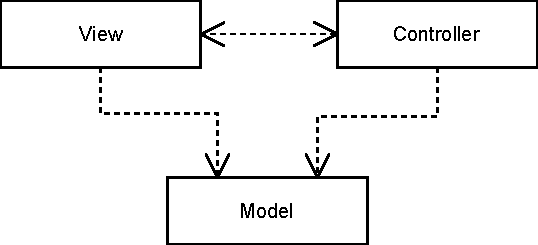
\includegraphics{figures/design-patterns-mvc-1.pdf}
    \caption{MVC overview}
    \label{fig:mvc-overview}
\end{figure}

\begin{figure}[htb]
    \centering
    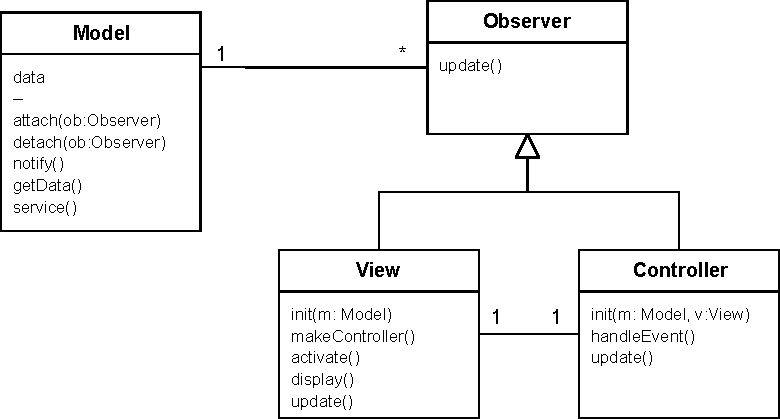
\includegraphics{figures/design-patterns-mvc-2.pdf}
    \caption{MVC with observer pattern}
    \label{fig:mvc-with-observer}
\end{figure}


\subsection{Common Patterns in the project}
DI, inversion of dependency, reveal, factory, async, fowler... hints of the remote façade and SOA¿?

This subsection is a high-level description of the most relevant software patterns in the project.

paragraphs for the patterns go here

\paragraph{Constraints}
FIXME this section sucks
%Flango Content Manager has  been designed taking into account the guidelines of \ac{GRASP} and the five basic principles of \ac{SOLID}.
The project follows object-oriented design adapted to the constraints induced by the technology and the requirements of the project.

FIXME improve this:
\begin{itemize}
    \item The \textbf{Angular Framework} is an approach to Web Components but components are not fully reusable. Moreover, most of the cl
    \item  Legacy \ac{XML}. The contents application uses \ac{XML} to define screens, templates, components, etc. The vocabulary and grammar of this \ac{XML} was designed having Adobe Flash and imperative programming in mind. While imperative programming is great for business logic, Angular prefers declarative programming for the view. 
%    \item This project is not a traditional \ac{CRUD} application. The model is a set of screens and 
\end{itemize}

% FIXME these are horrible paragraphs
\paragraph{\ac{GRASP}} The patterns used in \ac{GRASP} are: Controller, Creator, Indirection, Information Expert, High Cohesion, Low Coupling, Polymorphism, Protected Variations, and Pure Fabrication. 
Angular enforces a strict separation of concerns between components and together with \ac{TDD} and unit testing, it helps keeping components loosely coupled.
The framework provides an easy way to create Controllers, non-user interface objects responsible for receiving and handling events.
They are mediators between the model and the view (indirection pattern). 
For example, $ActionCtrl$ for buttons receive events from the \ac{UI} and delegate the action to the corresponding class.
New elements of the framework, like Services or Directives, are created using a factory function.
FIXME However, the model are the screens and instead of creating an object from an \ac{XML} file the system just appends it to the \ac{DOM} and defines the behaviour in Directives, the software hardly ever has to create instances of objects explicitly.
FIXME should this be here?: The model is stable during the execution of the application. That is, new instances of classes of the model can not be created. 
New instances of classes are hardly ever created because the model is stable during the execution of the application. 
Changes are not made persistent. The application retrieves the model, renders it and lets the user interact with the contents in the touchscreen.

\paragraph{\ac{SOLID}} Five basic principles in software design are present in this project.
Classes have a single responsibility (e.g. Configuration for the $palSettings$, or managing properties of \ac{UI} elements with $palProperties$). 
FIXME: This principle works well with unit testing.


\paragraph{Dependency Injection} One of the \ac{SOLID} principles, inversion of dependency, states that one should “Depend upon Abstractions. Do not depend upon concretions.”
QUOTE: Dependency Inversion is the strategy of depending upon interfaces or abstract functions and classes, rather than upon concrete functions and classes. This principle is the enabling force behind component design (http://www.objectmentor.com/resources/articles/Principles and Patterns.pdf) Robert C. Martin ('Uncle Bob'), objectmentor.com. Last verified 2009-01-14.
Dependency Injection is one of the implementations of this principle.
The framework encourages the use of this pattern in all components. 
Thus, services can be injected in controllers and directives.
Using the name and a service registry, the client class does not need to create an instance of the injected service. 
A particular implementation of this principle is in the wrapper for roslibjs: the service palROSBridge in the application is made injectable and provides callbacks to allow a decoupled desing. FIXME LANGUAGE.



\paragraph{Factory} Directives, controllers, services... are registered on modules. 
The $module.directive$ \ac{API} registers them. 
It takes a normalised name and a factory function that returns an object with the fields that can be exposed to classes that use it.
For example, a Directive Definition Object or a Service.

\paragraph{Revealing Module} \cite{Osmani:2012} Modules typically help in having the units of code for a project separated.
JavaScript does not support the concept of classes but it does support special constructor functions that work with objects. 
The $new$ keyword used in a call to a constructor function makes JavaScript instantiate the new object with members defined by that function.
Modules are a way to emulate the concept of classes.
There are several options to implement them. 
This project uses object literal notation (CROSS REF JAVASCRIPT)
The module pattern encapsulates privacy, state and organisation using closures (CROSS REF JAVASCRIPT).
With the Revealing Module Pattern the code of the module is simplified: all the methods are kept private and only a few of the engineer's choice are exposed at the end, while setting up the public \ac{API}

\paragraph{Remote Facade} FIXME: sure? do I have a remote facade in the app, in a controller?

\paragraph{Command} 
Sometimes requests are issued to objects without knowing anything about the operation being requested or the receiver.
The command pattern is a behavioural design pattern in which an object is used to represent all the information needed to call a method at a later time. 
It lets objects make requests of unspecified application objects by turning the request itself into an object.
This object can be stored and passed around like other objects \cite{GoF:1995}.
Other names are Transaction or Action Pattern  

\fref{fig:design-command-general} shows the class diagram for a traditional object-oriented programming language.
With JavaScript there are no abstract classes.
The approach that Osmani proposes is having only concrete classes with a common $execute$ method \cite{Osmani:2012} CROSS REF CODE EXAMPLE

FIXME include code design-command-1.js and design-command-2.js
With a simple controller (CROSSREF listing 1) one would call the methods in the object.
while this is correct, at the time the \ac{GUI} is built the \texttt{UI Component} does not know about the operations being requested.
For example, there is no way to define the behaviour for a \texttt{UI Component :: Button} click handler.
Only the contents application knows it.
By adding an \texttt{execute} method to \texttt{ActionCtrl}, used in \texttt{UI Components} that accept the tag \texttt{onclick} and \texttt{action}, methods can be called without knowing them CROSS REF listing 2

\begin{figure}[htb]
    \centering
    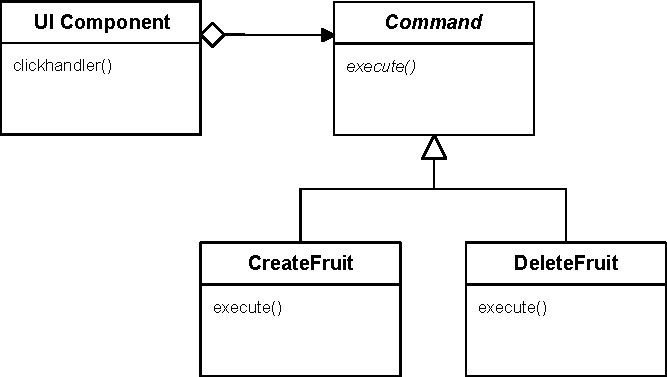
\includegraphics{figures/design-patterns-command-1.pdf}
    \caption{design patterns command 1}
    \label{fig:context-original}
\end{figure}

\begin{figure}[htb]
    \centering
    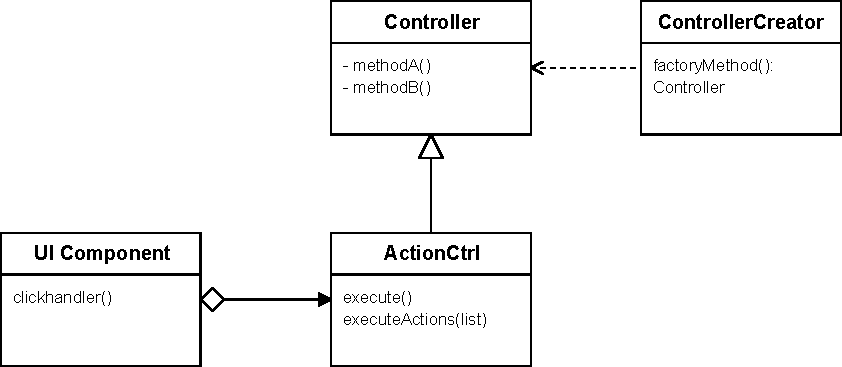
\includegraphics{figures/design-patterns-command-flango.pdf}
    \caption{design patterns command flango}
    \label{fig:context-original}
\end{figure}

\subsection{Orientation to Web Components}
Web Components is a set of specifications that let web developers use \ac{HTML}, \ac{CSS} and JavaScript to build widgets that can be reused easily and reliably.
A web component consists of five pieces\cite{W3CComponents:2013}:
\begin{itemize}
    \item \textbf{Templates} define chunks of mark-up that are inert but can be activated for use later.
    \item \textbf{Decorators} apply templates based on CSS selectors to affect rich visual and behavioural changes to documents.
    \item \textbf{Custom Elements} let authors define their own elements, with new tag names and new script interfaces.
    \item \textbf{Shadow DOM}  encapsulates a DOM sub-tree for more reliable composition of user interface elements.
    \item \textbf{Imports} defines how templates, decorators and custom elements are packaged and loaded as a resource.
\end{itemize}

At the time of developing this project, the specification of web components is still a work in progress.
The technology, however, seems to fit in the needs of the project.
There are 2 well-known initiatives that implement an approach to web components: Google Polymer and Google AngularJS.

\paragraph{Polymer} Polymer is a framework that aims to use Web Components. 
It's based on Custom Elements, i.e. everything is a component.
With Polymer developers can compose and encapsulate bits of HTML that can be used in any other templating system or framework.
It uses \ac{HTML} and the \ac{DOM} \acp{API} to separate the view (\ac{DOM}) from the model. 
Updates to the model are reflected in the \ac{DOM} and user input in the view is immediately propagated to the model:: fast two-way data binding.

Polymer is in pre-alpha stage and can not be used in a stable project.
Angular, the framework of choice for this project, has features close to web components: it has declarative templates (in directives) that can be applied for elements, attributes, comments or classes (like Web Components decorators).
Directives are custom elements: behaviour can be placed in a directive controller, in a compile or in a link function.
Templates are usually \ac{HTML}, although it is not shadow \ac{DOM}.
Units of code can be grouped in modules, services, etc and be reused.


\section{Static View}
the model, the view and the controllers. angualar modules, services, filters, controllers...
talk about the data model and \$rootScope ? talk about properties

un diagrama:
moduls, serveis, controladors, etc. 

\section{Dynamic view}
the flow: user creates an application, [robot sync], my app reads it and generates HTML output.

specific flow of an app. bootstrap, the compile-link phase, push classes, push styles, get url params, etc.
examples of using the properties, generating the settings, fetching things from the server, rostopics...

\section{Physical view}
robots, backend.basestation, wi-fi, vpn...

\section{External view}
there isn't! it's a backend app to create a frontend app.

\section{should there be any more sections?}
something more
